Based on the design of version 1


Based on the design of version 1, the current version is still a combination of the colour white (for the background) and orange (for miscellaneous design features). The white background leverages on its simplicity and clarify, this being an important criteria for retaining the attention of the user. Moreover, the orange colour is reportedly simulating for the users appetite. \footnote{[ http://desktoppub.about.com/cs/colorselection/p/orange.htm ]}. 

\begin{figure}[h]
\begin{center}
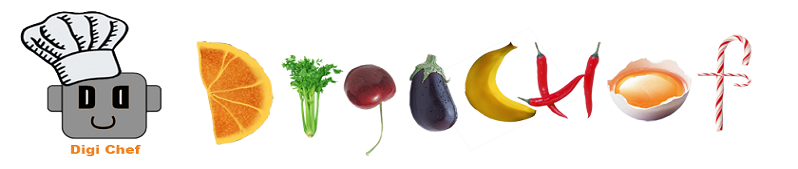
\includegraphics[width=0.9\textwidth]{logowebsite}
\caption{New Logo for Version 2}
\label{fig:logowebsite}
\end{center}
\end{figure}

The logo for version 1, however, has been replaced. The new logo ( Fig~\ref{fig:logowebsite} ) also uses the letters "Digi Chef" as the banner, but instead of just typing the banner in a simple font, we use several ingredients to sketch up these letters. Therefore, the logo can explain our website's main function, search by ingredients and you will get  recipes for delicious food. 

\subsection{Version 2}

Version 2 is an upgraded version of the original version containing more functions (described by the Product Specification). With the use of technology such as JavaScript, the web interface looks more professional. 

\begin{figure}[h]
\begin{center}
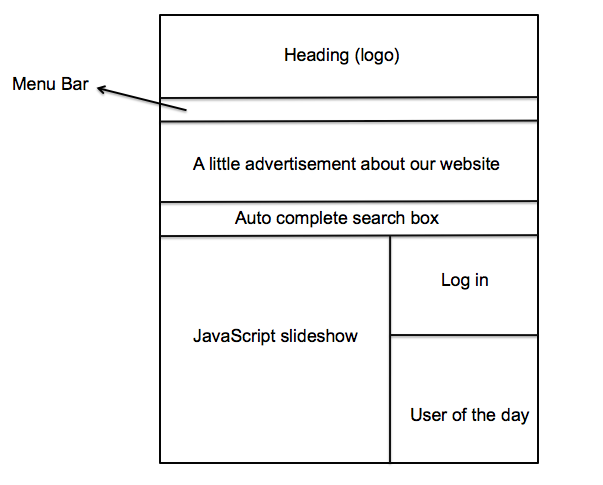
\includegraphics[width=0.9\textwidth]{home_page_v2}
\caption{Layout of the Home Page}
\label{fig:home_page}
\end{center}
\end{figure}

For version 2, our website has a larger database that contains over 900 recipes. For such amount of recipes it would be effort for the user is we were still using the drop down menu's for the search. Therefore, we have implemented a fancy search that auto completes text inputted and makes each ingredient a tag. 

\begin{figure}[h]
\begin{center}
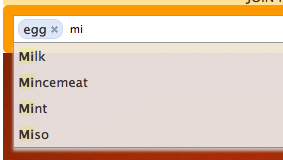
\includegraphics[width=0.6\textwidth]{auto_complete}
\caption{Auto Complete Search Box}
\label{fig:auto_complete}
\end{center}
\end{figure}

As shown in Fig~\ref{fig:auto_complete}, the user is able to search for recipes using more than three ingredients. When the user inputs an ingredient he/she is required to press enter to tokenise each ingredient. If the user wishes to remove the ingredient from the list, this is done by clicking the close icon at the top of the token. 

Furthermore, for version two, users are allowed to create their own account to rate the recipes. So a register section is presented in the right column of the website, below this section is a part that exhibits the user of the week. 

\begin{figure}[H]
\begin{center}
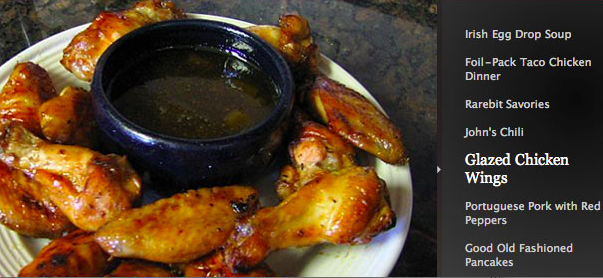
\includegraphics[width=0.9\textwidth]{slideshow}
\caption{Auto Complete Search Box}
\label{fig:slideshow}
\end{center}
\end{figure}

Fig~\ref{fig:slideshow} shows the JavaScript slideshow, the slideshow demonstrates a list of randomly selected recipes with their image and link.  

\begin{figure}[H]
\begin{center}
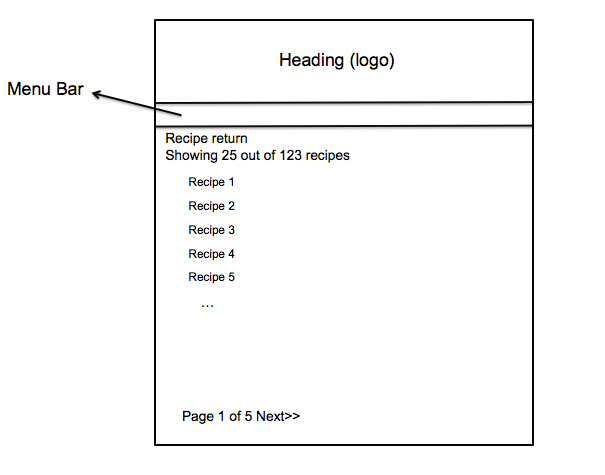
\includegraphics[width=0.9\textwidth]{result_list_v2}
\caption{Layout of the Recipe List Page}
\label{fig:recipelistv2}
\end{center}
\end{figure}

Fig~\ref{fig:recipelistv2} contains a list of returned recipes matching the list of inputted ingredients. Each recipe will contain at least one of the specified ingredients. Upon recipe selection, the specific recipe page will be displayed.  

\begin{figure}[H]
\begin{center}
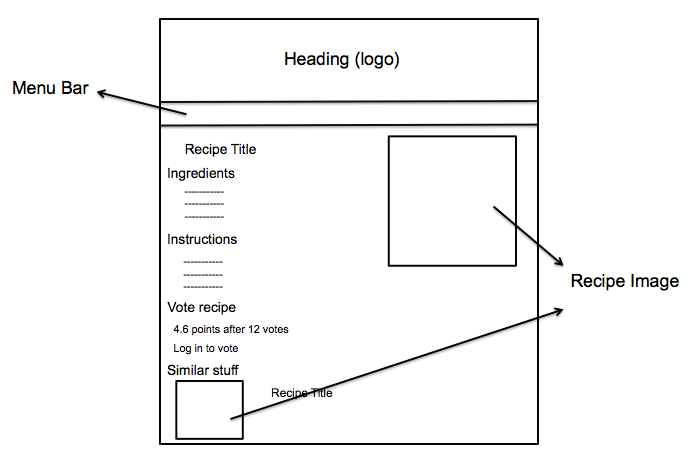
\includegraphics[width=0.9\textwidth]{recipe_page_v2}
\caption{Layout of the Recipe Page}
\label{fig:recipepagev2}
\end{center}
\end{figure}

The recipe page ( Fig~\ref{fig:recipepagev2} ) contains recipe details, this including the recipe name, an image, ingredients, instructions and the recipe tags. 

With the implementation of Collaborative Filtering we have included a list of similar recipes and the ability to like, hate or clear a vote when the user is logged in. The similar recipes section returns up to five related recipes together with their images. 

 
 \begin{figure}[H]
 \begin{center}
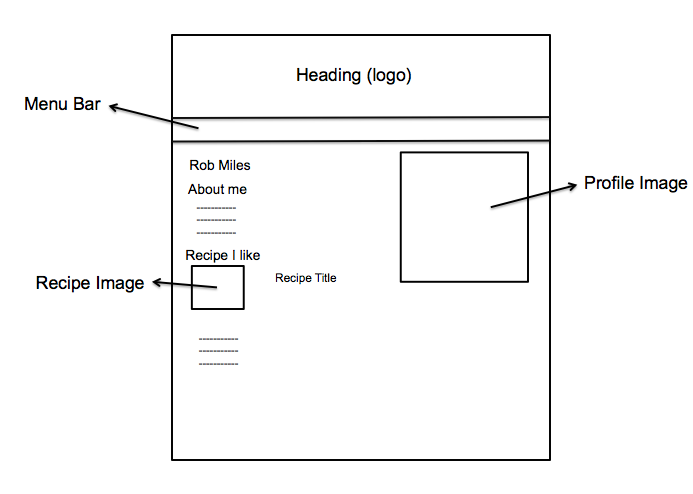
\includegraphics[width=0.9\textwidth]{profile_page_v2}
\caption{Layout of the Profile Page}
\label{fig:profilepagev2}
\end{center}
\end{figure}

When a user registers with Digi Chef, each user is provided with their own profile page (Fig~\ref{fig:profilepagev2}). The profile page includes an about me section and a list of recipes that the user has liked. 

\subsection{Version 3}



The ideal version of our product involves the implementation of a variety of possible functionalities. For instance, for the web based interface, users could choose to click tags and get a list of recipes that contains that particular tag. Additionally, recipes could be made searchable by not just ingredients but also, for example, the type of cuisine (Chinese dish) or whether recipes are vegetarian or non-vegetarian. Moreover, a mobile application could be developed. 

Social networking would be another possibility, with users being able to interact with other users and leave comments on the profile page as well as the recipe page. Users might be able to upload their own recipes and receive ratings from other users. The possibility for improvements are abundant.

